% !TeX root = ../main.tex
% Add the above to each chapter to make compiling the PDF easier in some editors.
\graphicspath{{./figures/ch1/}}


\chapter{Introduction}\label{chapter:introduction}

\section{Motivation}
Over the last two decades, auctions have been established as a reliable mechanism to allocate spectrum licenses to businesses that want to provide wireless communication services \cite{Cramton2002}.  Spectrum auctions already have produced billions in revenue for governmental institutions world-wide making it the preferred method of assigning spectrum. Well-designed auction mechanisms showed to be superior to previously used mechanisms like comparative hearings and lotteries, while maintaining the tendency to allocate licenses to parties that have the highest valuation for the bidding items \cite{Cramton2002}. 

When auctioning spectrum licenses, often certain license combination create an added value to the bidder. This may be induced by particular geographical arrangements or bundling of frequency blocks enabling new technology and thus produce a competitive advantage effecting the bidder's valuation of this item combination. In this case, the valuation of this bundling of items is greater than the sum of each item's valuation, which is called super-additive valuation. 

To achieve those desired combinations, in certain cases bidders might have to strategically bid over an item's valuation if it is part of such an item composition. Being uncertain if they can realise the desired bundling, the bidders \textit{expose} themselves, because they are still in danger of failing to achieve the combination and end up with single item prices that exceed their valuation.  
To overcome this issue, in combinatorial auctions bidders can place bids on item combinations. Nevertheless the helpful enhancement, the number of possible arrangements growths in combinatorial magnitude with the amount of items auctioned. Hence, finding the optimal allocation in an acceptable time frame becomes challenging as the calculations are computationally expensive and can lead to incomprehensible non-linear price progressions that are non-transparent for bidders. 

With the aim of constantly improving the performance of auctions, a wide array of different auction mechanisms were already devised over the last decades. Even though some formats prevail in their use in national spectrum auctions, academia and business partners are always in search for new solutions for questions arising in adopted auction formats, i.e. bidder exposure, non-linear and incomprehensible price calculations or computational complexity in combinatorial auctions.

The idea of hierarchical bidding was introduced by \citeauthor{Rothkopf1998} in 1998 and aims to reduce computational complexity in combinatorial auctions by structuring the bidding items into a hierarchy of pre-defined packages \cite{Rothkopf1998}. This gives bidders the opportunity to bid on a certain item combinations until their valuation. 
\citeauthor{Goeree2010} extended the idea of hierarchical package bidding by devising computation algorithms for the assignment and pricing of items with much less computational effort needed \cite{Goeree2010}. The goal of this thesis is to explore indicators of the eligibility of HPB in spectrum auctions by running simulations based on the German spectrum auction from 2015, which will be described in more detail in the following section. 

\section{The German Spectrum Auction in 2015}\label{sec:MBP16}
The German auction was conducted under the project name \textit{"Mobiles Breitband Projekt 2016"} by the German federal network agency \textit{("Bundesnetzagentur")} in 2015 over the course of 4 weeks or 181 bidding rounds and resulted in EUR 5.081bn of revenue. Germany, as the first European country, auctioned off the 700 MHz band to be used for mobile telecommunication purposes. The auction was important, as it offered valuable frequency bands ready to be used for expanding LTE coverage as well as prospective technologies and covered the spectra \textit{700, 900, 1800} as well as \textit{1500 MHz}, totalling in 270 MHz offered. In each band, a certain number of frequency blocks was sold in a 2 x 5 MHz fashion, except the 1500 MHz band, which was offered in 1 x 5 MHz blocks. During the auction, the blocks were treated as \textit{abstract} blocks, meaning that the bidder did not know the specific frequency allocation inside the band yet. After the auction, the blocks were then allocated to specific frequency values. With the exception of 1500 Mhz, the other bands each included one \textit{debased} block which was already tied to a certain frequency allocation due to technological circumstances (e.g. as buffer to other bands). \autoref{fig:freq-sold} shows the amount of frequency offered in each spectrum. 

\begin{figure}[h]
	\centering
	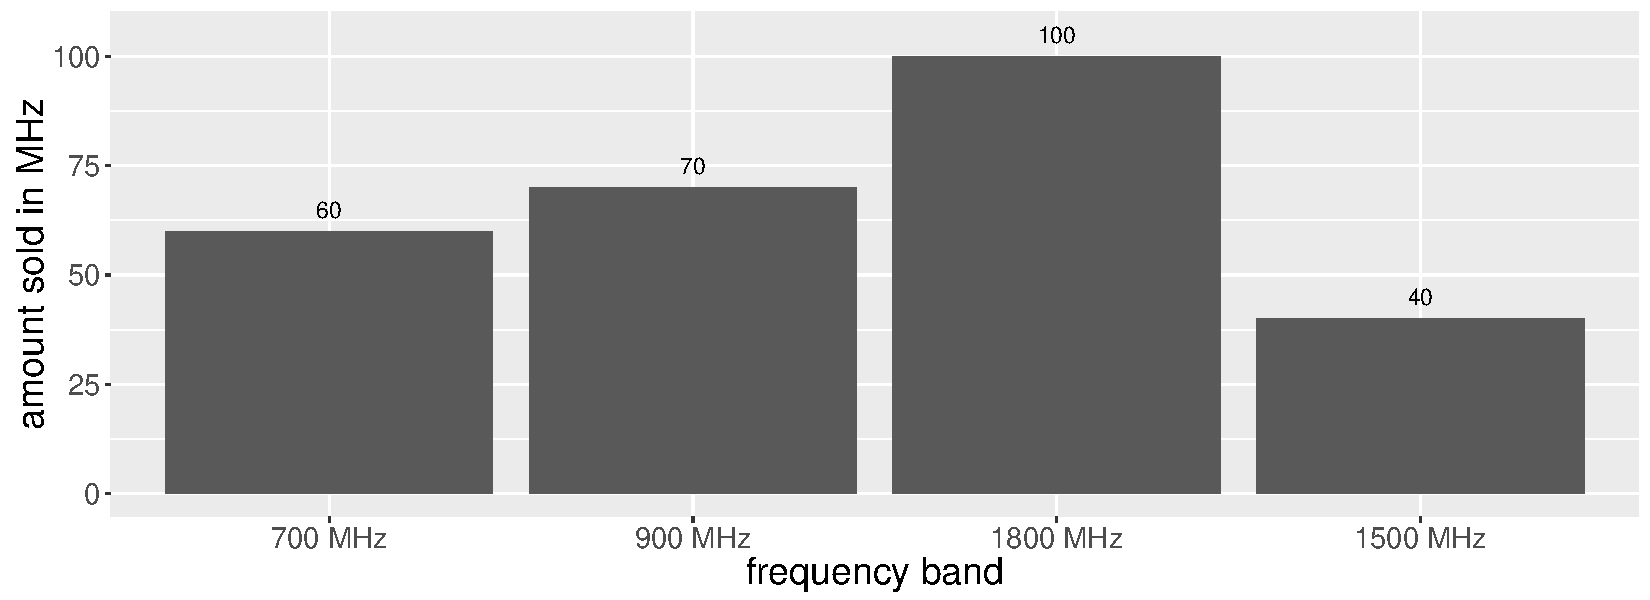
\includegraphics[scale=0.5]{freq_sold.pdf}\\
	\caption{Amount of MHz sold in the German auction} \label{fig:freq-sold}
\end{figure}

Since 2015, the German mobile network operator (MNO) market is split between three incumbent operators: "Deutsche Telekom AG" (DT), "Vodafone GmbH" (VOD) and "Telefónica Germany GmbH \& Co. OHG" (TEF). Just shortly before the auction, TEF merged with the German MNO "Eplus" reducing the number of active operators in the market. 

The auction format used was the Simultaneous Multi-Round Auction (SMRA). Including a set of different auction rules, the SMRA can be described as an extension of the English auction, where multiple items are auctioned \textit{simultaneously}: Each round, bidders place increasing bids and the auction stops when the bidders stop expressing new bids. After the end of the auction, every item is allocated to the bidder with the highest bid in the last round.
The specific implementation of SMRA differs from country to country. The German auction was standing out due to its high level of transparency. After every round, each bidder had access to a wide array of information, e.g. including the bids placed by every bidders. Thus, bidders were able to reconstruct the whole bidding history of every participating bidder and draw conclusions from the bidding behaviour. The data made available by the German federal network agency included only the highest bids placed and the current winner of each item, but was still valuable for deducting bidding behaviour.
Due to the available data and the low number of bidders, the German auction seemed like a suitable basis for the simulation done in this thesis.


%TODO vielleicht noch endresults rein?

\section{Contribution}
To contribute to the vector of improvement, this thesis is set-up to research the potential eligibility of the Hierarchical Package Bidding format (HPB) in the realm of national spectrum auctions by running simulations based on data from the German auction in 2015. The key questions that guided the process of this thesis can be summarised as follows:

\begin{itemize}
	\item By introducing pre-defined packages for bidders, can HPB provide significant progression in terms of efficiency and revenue of the auction?
	\item How does the set-up of the HPB bidding hierarchy influence the results?
	\item How \textit{"stable"} is the format in comparison to the well established Simultaneous Multi-Round auction format? 
\end{itemize}

To find answers to those questions, I extended an existing project from the university chair and introduced the specific characteristics of the German auction into the implementation, as well as improvements on existing program code. Accordingly, I derived a value model to describe the valuations of the agents in the simulations. Also, I needed to devise a selector model that let the bidders emulate an optimal bidding behaviour under the constraints of the German auction. To set-up the HPB simulations I developed two different hierarchy structures to explore their effect on the performance of the auction. 
On the basis of this work, I ran several simulations with different parameter configurations to research the performance and stability of HPB in comparison to SMRA.

\section{Thesis Outline}
This thesis is organized as follows: \autoref{chapter:theory} introduces important concepts and terminology of auction theory as well as establishes an understanding of the auction formats used in the simulation. Subsequently, \autoref{chapter:experiment} first gives an overview of the data from the German auction. Based on the insights gained from the analysis and external sources I  than devise a value model to describe the bidding behaviour of the agents in the simulation. The following \autoref{chapter:simulation} is the heart of this thesis, comprising of the explanation of the simulation process and a description of the results. Lastly, \autoref{chapter:conclusion} draws final conclusions from the simulation data and gives an outlook for future work.


%BACKUP
%If bidders can only place bids on single items, but have item combinations that posses a super-additive valuation, meaning their valuation is higher than the sum of the items' valuation, they might feel incentivized to bid over a certain item's valuation in order to realise a desired bundling. This is called the exposure problem. In case the bidder fails to acquire this arrangement, it runs into the risk of paying prices that exceed the valuation of the item. 
